
\section{Methodology}

As discussed, the market type for the artifical market was chosen 
to be continuous double auction or more specifically limit order market.
The artificial stock market created in this thesis was written in Julia
programming language and it took some inspiration from previous literature.
The literature is lacking on practical studies about how to actually create
an artifical stock market and therefore the actual structure of the market is explained
in depth. The decisions about the microstructure and the trader behaviour
is most closely to the work of \citet{Genoa01} and \citet{Raberto05}
whereas for the structure and practical implementation the inspiration
was taken from the work of \citet{Ben12}. The goal was to create a generic artificial market 
model with empahsis on flexibility and practicality. Many of the features
of the model are not tested in this thesis because of the scope of the thesis.
The plotting and analysis of the results were conducted using Python and its scientific
computing stack including Numpy, Pandas, Statsmodels, Matplotlib, Seaborn and Scipy library.
In this section the rationale for the programming choice of the model is discussed
and its structure, mechanics and generic characteristics are 
explained.


\subsection{Julia Language}
Julia is relatively new dynamic programming language, 
reaching stable release of 1.0 in August 2018 \citep{JuliaV1}.
It is a performant language with an empahsis
on productivity. Even though Julia has a focus on scientific 
computing it considered as a general purpose programming
language. Some of its features include
multiple dispatch, just-in-time compilation and built-in
matrix data types \citep{Julia}.

Julia fits well in building an artificial market.
Artificial markets can be seen as sets of objects
and interactions in between, as described \citet{Ben12},
and in such models object-oriented programming (OOP)
is preferred. Even though Julia is more functional in nature, 
features of OOP could be constructed with Julia's mutable structs 
and type annotated functions. Also, the speed of code execution, 
support for matrix operations and good productivity makes 
it viable language for prototyping simulation systems. 


\subsection{Generic Structure of the Model}
% Describe the generic structure (Type hierarchy, layers etc.)
% Kind of the static side of the simulation
The ASM model has three layers: abstraction layer, concrete 
layer and simulation layer. The fist layer, abstraction layer, contains the 
generic parts of the framework that are independent and obvious in terms
of functionality. For example, how to get traders' positions, how to
transfer assets from a trader to another or how to cancel an order are
functionalities that are independent on the type of the traders 
and type of the markets and therefore these functionalities have little
far reaching decisions to make. The main purpose of this layer
is to separate generic and obvious functionality from blocks of code
that has more degrees of freedom and less obvious decisions to make.

The second layer, the concrete layer, defines the actual types and
functionalities that require less clear and more heuristic
approach than the abstract layer. This layer also include significant
portion of choices to make. Some of the components
on this layer include the zero intelligent trader and its
functions that defines its behaviour, the continuous double auction
market and its price formation mechanics.

The third layer, simulation layer, manages the simulation as a whole.
This layer defines the ecosystem where the simulation takes place including
the initiation of the components, interating over the time periods, asking
each trader to make their decisions and ask the market to clear. 
Also, the number of investors, initial conditions such as amount of assets 
the investors own and how the simulation results are saved are defined here. 
This layer mostly calls the functionalities created in the lower layers.



\subsection{Simulation Process}
% Describe how it works, how the dynamics flow etc.
In functional sense, the model consists of three main components:
the main level code, traders and markets. The main level code 
orchestrates the flow of the simulation while traders and markets
handle the pieces of functionalities associated with them. The process
is generalized in ~\ref{fig:sim_proc}. The beginning and the end of the 
simulation are shown in orange in the figure. Yellow boxes represent
the actions that belongs to the concrete layers and all the actions that
are in the main are part of the simulation layer. The remaining belong
generally to the abstract layer.


\begin{figure}
    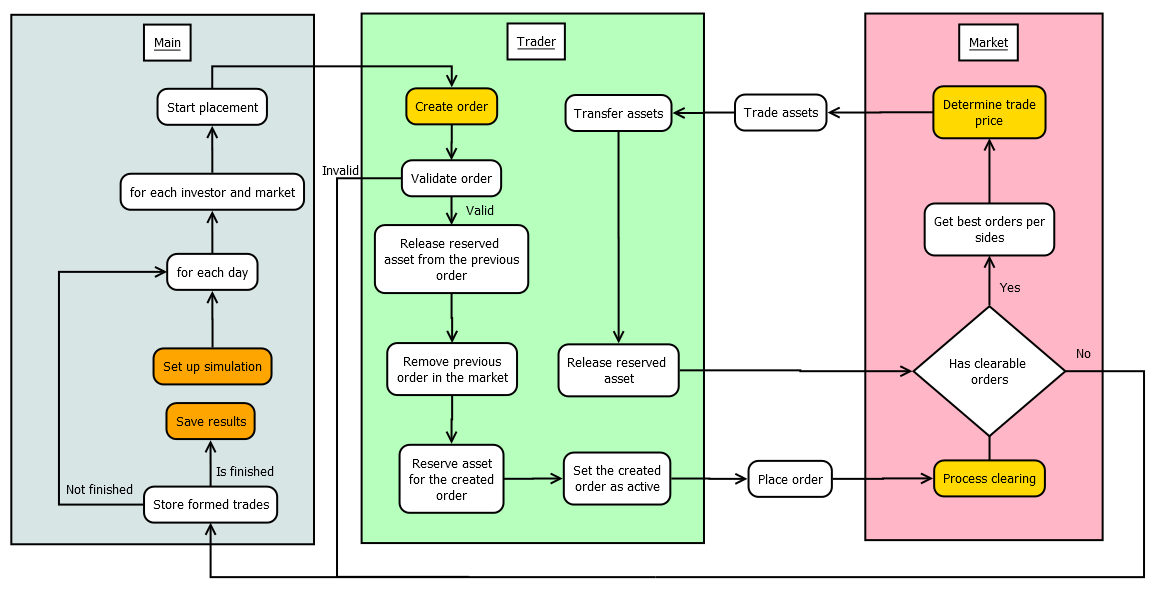
\includegraphics[width=\linewidth]{diagrams/placement_clearing_process.png}
    \caption{Simulation process}
    \label{fig:sim_proc}
\end{figure}

The simulation begins with setting up the parameters such as number of
trading days and initializing the traders, their assets and the markets.
Then each trading session is iterated in which each trader can create order 
an order to each market. After the order creation the order is validated.
The traders have also an option not to create an order. If the order was
valid, the previous order to the market is cancelled and the needed 
asset is reserved for the order in case it executes. The asset
reservation is to prevent traders going over their budgets if they
have allocated the same asset in other markets. Next the order is
placed to the market and the clearing process begins in case of 
continuous double auction market. If there are any clearable orders,
they are traded with a price defined by the market type. When
all clearable orders are cleared, the process returns to the
main block and either next trading session is started or the next
trader gets chance to make orders. In this section, the process how the
zero intelligent traders conduct their decisions and how the 
market price formation and clearing works is discussed with more detail.
There are some interesting characteristics in the asset dynamics of this
artificial market and these are also discussed.

\subsubsection{Trader Behaviour}
% How the investors make decisions actually

As mentioned, the traders of the ASM model are zero-intelligent
traders. The reason for this is to minimize the degrees of freedom introduced with
the model and provide as generic structure as possible. The traders' rationality 
for making decisions is reduced to minimum effectively making them unable to speculate, 
manage risks or optimize portfolio. They do not possess ability to seek profit, 
observe the markets or learn from their previous actions or peers and
they are only able to submit random orders. The mechanics of zero-intelligent traders
are implemented in a way that they are given sets of allowed ranges 
and options in which they choose values randomly. This way the zero-intelligent behaviour is maintained
in addition to have similar options that there are present in real markets 
concerning to order placement such as the order quantity, order price and whether
to submit an ask order or bid order. The traders are also budget constrained
in order to achieve allocative efficiency as proposed by
\citet{God93}.


An order placement decision in the model requires three components 
to be defined by a trader: order side, order quantity and order price. 
There are obviously two possible sides of an order: bid and ask, but
not submitting an order is also a choice. Therefore, the traders
have three options: submitting bid limit order, submitting ask limit order
and not submitting an order. Submitting an order also cancels any previous
order made by the trader to the same market but not submitting an order doe not. 
The traders pick one of these options randomly and each option has equal weight. 

Determining the order price and order quantity are not as straight
forward as their feasible ranges cannot be determined completely independently
from each other and the calculation of the ranges differ between bids and asks. A bid order's
value cannot exceed the amount of currency the trader possess thus this is 
a limiting factor for both, order quantity and order price of a bid. In addition,
the maximum order quantity is inversely proportional to the order price and
therefore if order price is set first, the maximum order quantity the trader
can set for a bid equals to its amount of currency divided by the price and vice versa. 
However, the ask order does not include such restrictions: the value of the order
does not reflect to the amount of assets the trader must allocate for the order. The
price of an ask order can, in theory, be infinite and the trader has no issues
fulfill the trade even though the counterparty may have. The only limit for the
trader placing an ask is the amount of the traded asset it possess: the trader
cannot sell more of the asset than it has. To summarize, an ask order's feasible
ranges for quantity and price can be determined independently but this is not the
case for bid orders. These feasible ranges are shown in ~\ref{eq:feasible_ranges}.

\begin{equation}
\begin{aligned}
% Bid
p_{bid} &= \left[1, pos_{ccy} / q \right] \\
p_{ask} &= \left[1, \infty \right] \\
q_{bid} &= \left[1, pos_{ccy} / p\right] \\
q_{ask} &= \left[1, pos_{asset}\right] \\
\end{aligned}
\label{eq:feasible_ranges}
\end{equation}

To overcome this and to maintain symmetricity between the placement of bids and asks, 
the traders decide the amount of an asset to allocate with an order instead of deciding 
the order quantity directly. This decision is independent on the order price for both
sides and can be handled the same way for both cases. Therefore a trader placing a bid order 
need to define the amount of currency to allocate with the trade and a trader placing an ask
order need to define the amount of the traded asset to allocate, the order quantity in this case. 
The order quantity for a bid is calculated after the amount of asset to allocate 
and the order price have been set. The amount of asset to allocate is drawn from a uniform
distribution in which the minimum is one and maximum is the amount of the asset the trader
has and is free for allocation. The order price is drawn from a normal distribution in which 
the mean is the last market price. The standard deviation of the distribution is set to a 
constant and the distribution is truncated between one and infinity.

% TODO: Show and discuss about the ranges of the orders

An example of the distribution of order prices and quantities
is show in ~\ref{fig:generated_orders}. The figure contains simulation
of 1 000 000 orders created by a zero-intelligent trader. 
The last market price was set to 1 000 units and the standard deviation of the price to 10. 
The trader possessed 10 000 000 units of currency and 100 000 
units of stock.

\begin{figure}
    \centering
    \begin{subfigure}{.5\textwidth}
      \centering
      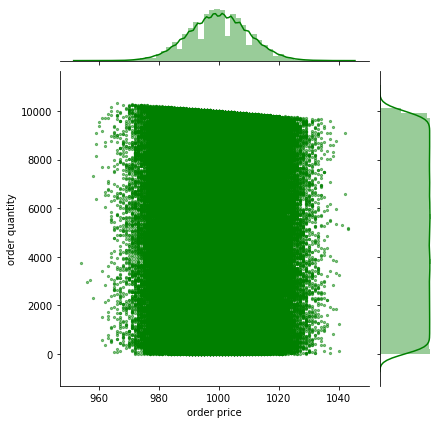
\includegraphics[width=\linewidth]{plots/order_distr_bid.png}
      \caption{Distribution of random bids}
      \label{fig:gener_bids}
    \end{subfigure}%
    \begin{subfigure}{.5\textwidth}
      \centering
      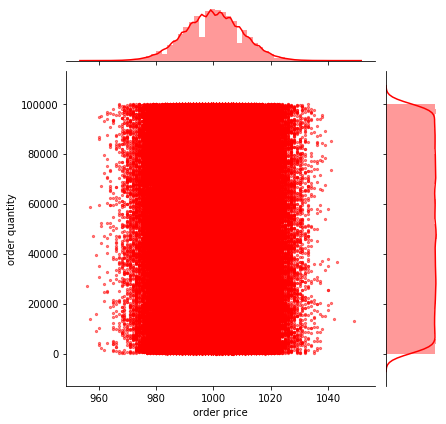
\includegraphics[width=\linewidth]{plots/order_distr_ask.png}
      \caption{Distribution of random asks}
      \label{fig:gener_asks}
    \end{subfigure}
    \caption{Distribution of random orders}
    \label{fig:generated_orders}
\end{figure}



In the literature, zero-intelligent traders are often implemented differently. For example, in the studies conducted by 
\citet{God93}, \citet{Jam96} and \citet{Mil08} the traders were initially divided to buyers and
sellers, traders could only trade one quantity of a stock per order and the prices
were drawn from uniform distribution. However, these markets did not aim for
realistic market microstructure. The trader behaviour in this model is close with the Genoa Market
created by \citet{Genoa01} as in this model the prices are also drawn from normal distribution and
the order quantities are derived from the required amount of asset. However, in Genoa Market the
normal distribution's mean is 10\% higher for ask orders and 10\% lower for bid orders from the
latest market price due to increase liquidity. For maintaining simplicity, the mean of the distribution
is set to the last market price in this mode. Also, the option of to not make an order seems not to be
implemented in the literature. However, \citet{Raberto05} implemented waiting times and order cancellation
after specified times which may produce similar behaviour. 

\subsubsection{Time Handling}
% TODO
The time in the simulation took inspiration from the asynchronous model created by \citet{Julien07}. 
As in their ASM model, in this model the traders are randomly given the ability to speak and make 
their trading decisions. The 

\subsubsection{Market Mechanics}
% How the market is cleared actually 

The market is continuous and double auction in nature.
The clearing mechanics themselves are, however, 
rather the same as could be for a call market: 
the orders are cleared until there
are no bid orders with price equal or exceeding the
ask order with lowest price. 
Continuity is achieved by launching the clearing process
every time an order arrives to the market. 
The clearing mechanics are defined in 
the abstraction layer in a way that the same body
of code works for call markets and continuous markets
and the distinction between the markets, such as how 
the market price is formed, is handled inside the clearing
mechanics by calling the parametrized functions that are 
defined explicitly for each concrete market type. 
The main body of the clearing function, 
as written in the source code, is shown in the listing ~\ref{lst:clearing}.
In the listing the clearing price resembles the market price
of the clearing session which is calculated in call markets but not in
continuous markets. This is so that in future experiments
that study call markets could utilize the same code without modifications 
even though call markets are not studied in this thesis.


\begin{lstlisting}[caption={Clearing process},label={lst:clearing}]
...
# The clearing price is defined here
# in case of call market. Nothing
# should be returned if the price
# is defined per order pair basis
clearing_price = get_trade_price(market)
while maxprice(buy_book) >= minprice(sell_book)

    order_sell = get_best(sell_book)
    order_buy = get_best(buy_book)
    
    # trade_price is clearing_price if defined,
    # else calculated per order pairs
    trade_price = (
        ~isnothing(clearing_price) ? 
        clearing_price
        : get_trade_price(order_buy, order_sell, market=market)
    )

    trade = trade!(
        order_buy, order_sell, 
        price=trade_price, 
        from=market.currency, 
        to=market.traded_asset
    )
    ...
\end{lstlisting}

The price formation of the continuous market is implemented
on the order pair basis. The trade price is simply the price
stated in the older of the paired orders. % SOURCE: find a source to describe why this way the price
The quantity of the trade is chosen from the smaller of the two orders
and the bigger order is partially cleared in case they were not 
equally sized.

% About literature


\subsubsection{Handling of Assets}
% Why use integers as units for assets

The model is constructed in a way that enables usage of multiple assets
and the assets are handled symmetrically. The former is achieved with
allowing multi-asset positions and it is the simulation layer's 
responsibility to decide the assets, markets and ask the investors
to create orders on them.

The asset symmetricity means that there is no universal or central currency 
and the currencies are handled as any other asset. In theoretical sense, 
currencies are also just investment options and there is no inherent reason why other 
asset classes, such as stocks, could not operate as the definition 
of value. This feature creates complexity to the model compared to a model
with a central currency acting as a baseline but it also enables an
abstracted structure that handles natively cross currency
markets or ecosystems where there exists markets between assets A and 
B and between B and C but not between A and C. It is also a better 
representation of theoretical markets.

Asset symmetricity is constructed via storing all the owned and reserved
assets in the same data structures, in dictionaries in this case. In addition
to the traded asset, the markets contains also the information about the asset
that the traded asset is traded with, which is most often some sort of currency. 

% Asset allocation, reserve & active orders
In single asset markets where only one order is allowed to be on the markets
per trader, disallowing orders that would require more assets to execute
than there is in the position should be enough. However, in case of multi-market
ecosystem this is not enough. The assets that are already allocated to 
a market must be kept track of. There most likely is a structure in a multi-market
simulations where the same asset is traded in more than one markets. If the
total commited amount of the asset is not tracked, there is a risk that the
same asset is commited in two separate orders and if both executes,
there is a chance that the trader's position goes negative. To prevent this,
this ASM model keeps track of all of the commited assets, called reserved
asset in the simulation, in addition to the actual position values. It also
accepts only one order per trader per market as it makes little sense that
the traders are allowed to express multiple different opinions to the market 
simultaenously: especially having a bid and an ask orders on the same market
at the same time may lead to a confusing pattern where a trader is trading with
itself. 

In addition to this, the order that a trader has already placed
to a market is tracked in the trader's data structure to make cancellation easy
but also implement relevant additional feature: active order lookup. To prevent that
the placing of a new order is not limited with the trader's existing order in the market,
the effect of this previous order, called active order, in the asset reverse is excluded. 
This active order will be cancelled as soon as the this new order is validated and this new order
will become the active order thus it is not a valid reason to make the trader's placing 
options more conservative.

% Integers & bid-ask asymmetricity
All quantities of assets are stored as integers to prevent wealth leakage
or creation because of the floating point arithmetics. Using integers also
conveniently act as the tick size for all the markets. This also has the side effect
of that also all the prices must be represented as integers as one piece
of traded asset must equal exact quantity of the asset used as a currency
in the market. Furthermore, this creates deficency in the market if the quantities
of owned assets are small and also a phenomenon of asymmetricity between bidders and askers
araises. The price set by an asker can be virtually anything: they can set
arbitrary positive price for their order as the only limitation is the amount
of traded asset they can commit to the order which is independent on the price. 
Every unit of increase in order price means more profit for the seller
in case the order is executed. On the otherhand, because of the 
lower limit of one in price the bidder does not have the same freedom.
The maximum price the bidder can set equals to the quantity of the asset
that behaves as currency in the market but the minimum price is one. This is
illustrated in the figure ~\ref{fig:buy_sell_asym} in which the all possible
combinations of quantities and prices are shown. The buyer owns
ten units of currency and the seller respectively owns ten units of traded stock in
this example. The colored areas represent where the possible combinations
lie.
 % And what this causes etc.
 % Price can be anything for seller but for buyer, there are boundaries

 \begin{figure}
    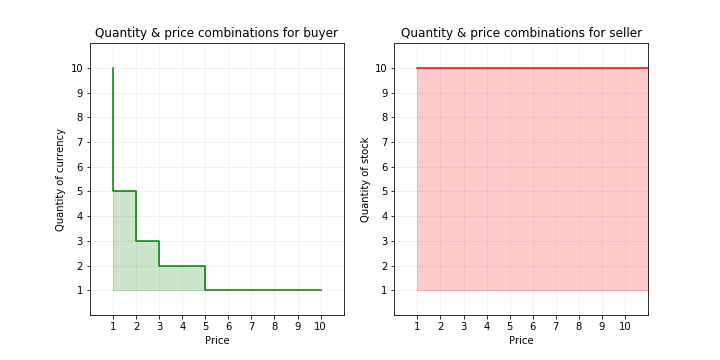
\includegraphics[width=\linewidth]{plots/buyer_seller_asymmetricity.png}
    \caption{Illustration of buyer-seller asymmetricity}
    \label{fig:buy_sell_asym}
\end{figure}

The bid-ask asymmetricity may become issue when the price of the market
approaches one. Near one the tick size start to reduce the efficiency
of the markets: for example, only one tick drop for a market price 
of four is 25\%. In addition, there may be an issue that the efficient
price cannot be reached if it lies under the price of one. Probably
the simplest solution to avoid this while still having integers for quantities 
of assets is to make sure the traded asset has sufficiently high value
compared to the currency of the market. This can be achieved simply injecting
enough currency to the ecosystem to inflate the price. Another interesting 
solution to solve the problem of the potentially unreachable efficient price 
is to have two markets for the same asset pairs but opposing direction. 
The first market trades an asset A with an asset B but the 
other market trades the asset B with the asset A. The price of the other market
should always be multiplicative inverse of the other so the.
This solution is shown in the figure ~\ref{fig:opposing_markets}. The total
amount of stock is increasing, thus inflating, and the total amount of
currency is decreasing, thus deflating, in constant rates.

\begin{figure}
    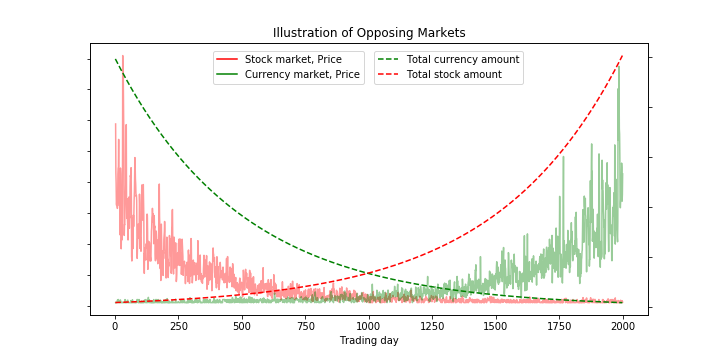
\includegraphics[width=\linewidth]{plots/opposing_markets.png}
    \caption{Two markets with inverse assets}
    \label{fig:opposing_markets}
\end{figure}


The efficient price of the market cannot be reached if it
lies below one. Therefore the simplest solution to the problem probably
is to make sure that the price of the traded asset is never close to one
To avoid any side effects from the bid-ask asymmetricity, there are two solutions:
either have two opposing markets for same asset pairs or have a balance between the 
assets in a way that orders with a price of one are unlikely. 
% implmenentation of payoffs (dividend, interests etc)

% How the literature
%Most of the ASM literature study only ecosystems in which
%the traders can only trade a stock with a cash.